\documentclass[a4paper, 12pt]{article}

% osnovni paketi za jezik in kodiranje znakov
\usepackage[slovene]{babel} 
\usepackage[utf8]{inputenc}
\usepackage[T1]{fontenc}
\usepackage{lmodern}

% dodatni paketi
\usepackage{amsmath, amssymb, amsthm}
% \usepackage[font=small, center]{caption}
\usepackage[hidelinks]{hyperref}
\usepackage{graphicx}
\usepackage{wrapfig}
\usepackage{float}     
\usepackage{geometry}
\usepackage[table]{xcolor} % http://ctan.org/pkg/xcolor
\usepackage{biblatex}
\addbibresource{literatura.bib}


\begin{document}

\begin{titlepage}
    \begin{center}
        \large
        Fakulteta za matematiko in fiziko\\
        Oddelek za matematiko \\
        \vspace{6cm}
        \Huge
        \textbf{Vizualizacija Kakeya-množice} \\
        \vspace{6cm}
        \large
        Terezija Krečič\\
        Pedagoška matematika, 5. letnik\\
        \vspace{1cm}
        Predmet: Matematika z računalnikom \\
        Mentor: Sergio Cabello\\
        \vspace{2cm}
        Ljubljana, 21. 5. 2024
    \end{center}
\end{titlepage}

\newpage


%%%%%%%%%%%%%%%%%%%%%%%%%%%%%%%%%%%%%%%%%%%%%%%%%%%%%%%%%%%%%%%%%

\section*{Uvod}

V tej projektni nalogi je bil cilj vizualizirati Kakeya-množico s pomočjo programa \href{https://ipe.otfried.org/}{Ipe}. Najprej sem morala sploh predelati problem, ki ga je zastavil Kakeya več kot 100 let nazaj, poleg tega pa se še spoznati z novo programsko opremo.

V poročilu bom na kratko predstavila glavno vprašanje in eno strategijo, kako ga rešiti. Vse slike, ki so vključene zraven, sem ustvarila sama s pomočjo Geogebre in omenjenega orodja Ipe. Poročilo je izhaja iz Besicovitchevega članka~\cite{Besicovitch}, vendar sem nekaj delov poenostavila in predelala.

%%%%%%%%%%%%%%%%%%%%%%%%%%%%%%%%%%%%%%%%%%%%%%%%%%%%%%%%%%%%%%%%%

\section*{Kakeyev problem igle}

Japonski matematik Sōichi Kakeya je leta 1917 zastavil naslednje vprašanje, ki se ga je v kasnejšem času prijelo ime ``\emph{the Kakeya needle problem}\footnote{Kakeyev problem igle, op. prev.}'':

\vspace{0.2cm}
\begin{center}
    \textbf{Kolikšna je lahko najmanjša ploščina območja, znotraj katerega se daljica dolžine 1 zvezno obrne za 180°?}
\end{center}
\vspace{0.2cm}

\noindent Poglejmo si tri primere geometrijskih likov, ki ustrezajo pogoju iz vprašanja:

\begin{enumerate}
    \item krog s premerom 1 $ \rightarrow $ ploščina $ = \frac{\pi}{4} \doteq 0{,}79 $
    \item enakostranični trikotnik z višino 1 $ \rightarrow $ ploščina $ = \frac{1}{\sqrt{3}} \doteq 0{,}58 $
    \item deltoida\footnote{za konstrukcijo deltoide gl.~\cite{deltoida}, za animacijo obračanja igle znotraj nje pa~\cite{kakeya_wiki}}, včrtana v krog s premerom $ \frac{2}{3} $ $ \rightarrow $ ploščina $ = \frac{\pi}{8} \doteq 0{,}39 $
\end{enumerate}

\begin{figure}[h!]
    \centering
    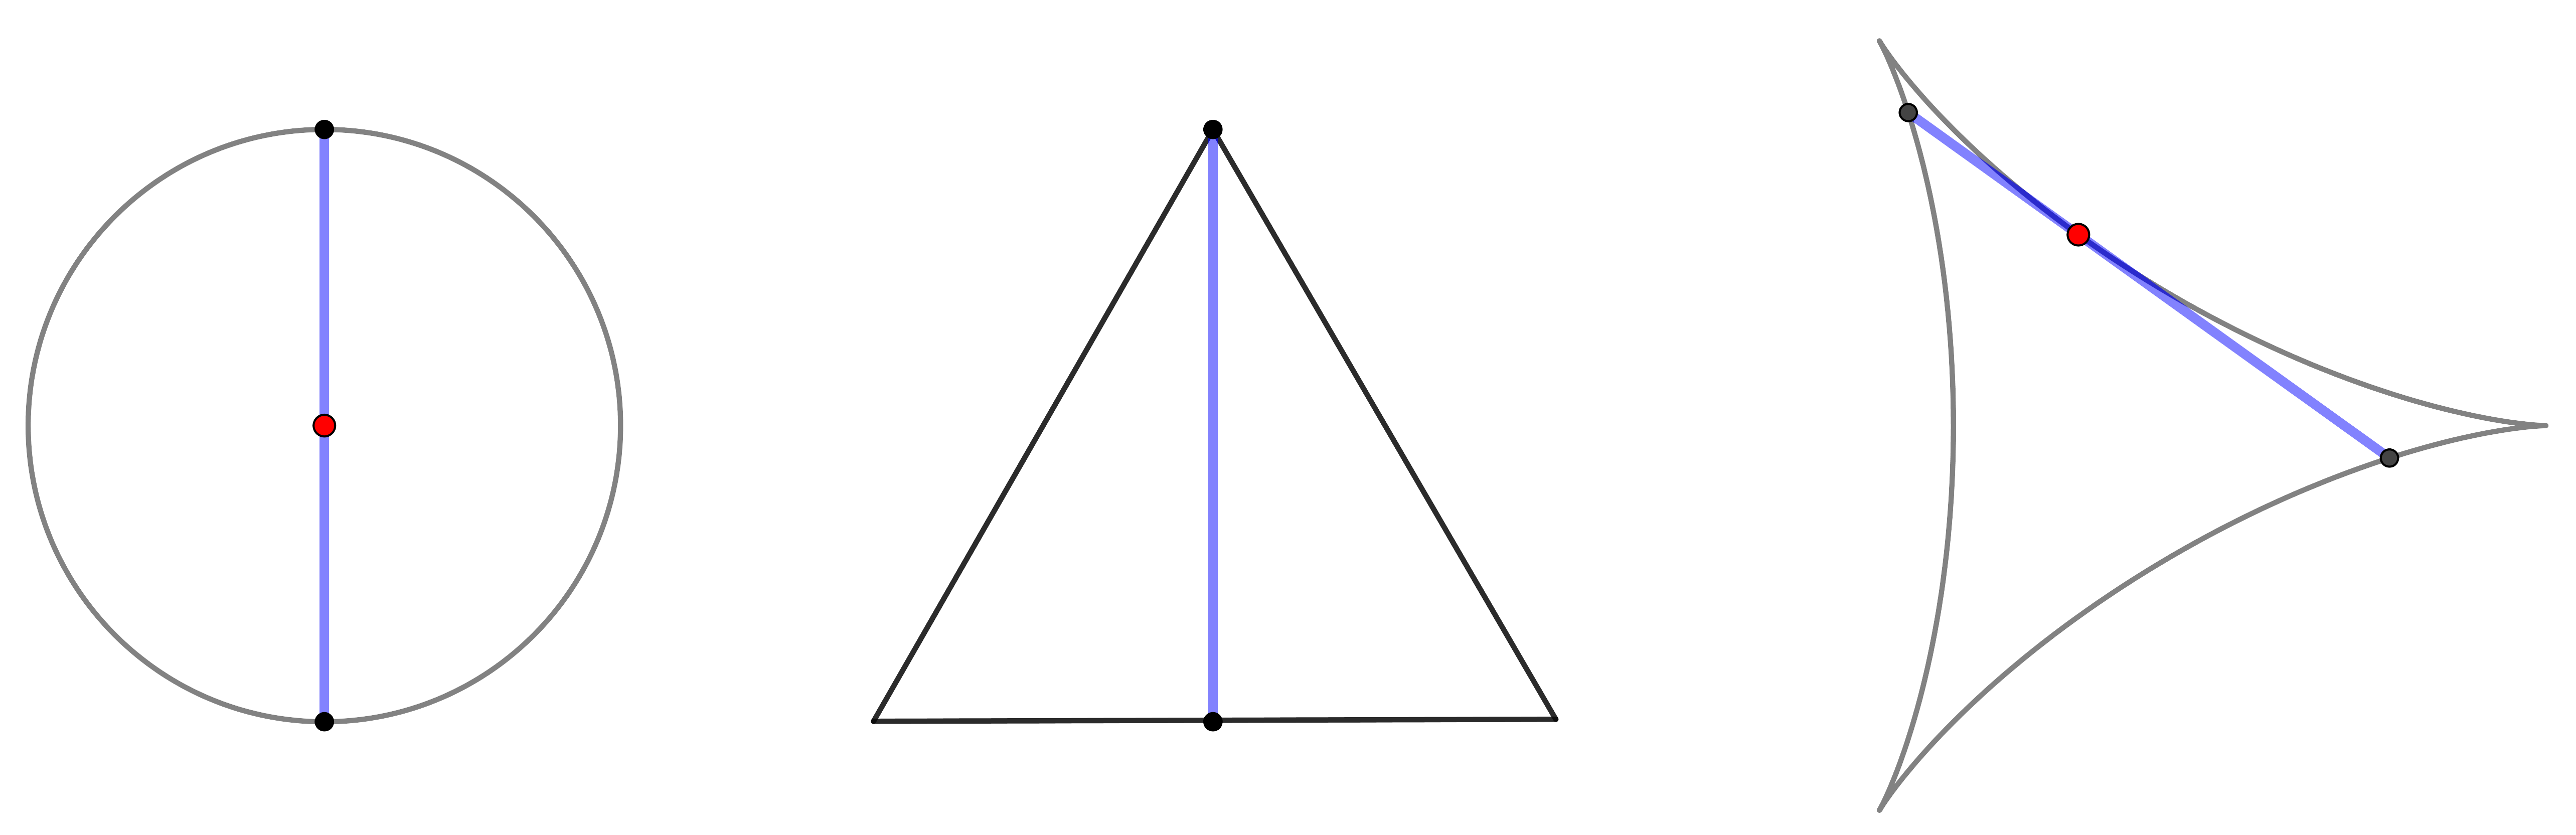
\includegraphics[width=0.9\textwidth]{geogebra_slike/prevelike_ploscine.png}
    \caption{Primeri, ki ustrezajo pogoju.}
    \label{primeri}
\end{figure}

Nekaj časa je veljalo, da je tretji primer, tj. deltoida, odgovor na vprašanje Kakeye, vendar je ruski matematik Abram Besicovitch uspel dokazati, da \textbf{spodnja meja za iskano ploščino \emph{ne} obstaja}. K enostavnejši konstrukciji primera takega lika je pripomogel tudi nemški matematik Oskar Perron, svoj del pa prispeval še madžarsko-danski matematik Gyula Pál.

%%%%%%%%%%%%%%%%%%%%%%%%%%%%%%%%%%%%%%%%%%%%%%%%%%%%%%%%%%%%%%%%%

\section*{Ideja za konstrukcijo}

Vzemimo enakokraki pravokotni trikotnik s katetama dolžine 2. Če v središče hipotenuze postavimo en konec enotske daljice, lahko njen drugi konec opiše kot 180°, ne da bi kakršenkoli del daljice zapustil trikotnik.

Ta trikotnik sicer ustreza pogoju iz vprašanja, vendar je njegova ploščina enaka 2 in večja od vseh treh zgornjih primerov.
Sedaj ga razdelimo na pol, kot kaže slika~\ref{trikotnik_razdelitev}, ter vsakega izmed delov (ki sta še vedno enakokraka pravokotna trikotnika) še dodatno razdelimo na $ n $ manjših trikotnikov z osnovnico dolžine $ \frac{2}{n} $ in višino 1. Enotska daljica se tako obrne za 180°, ko se v enem krajišču zasuče čez vrh vsakega izmed malih trikotnikov in prehaja med njimi preko skupnih stranic.

\begin{figure}[h!]
    \centering
    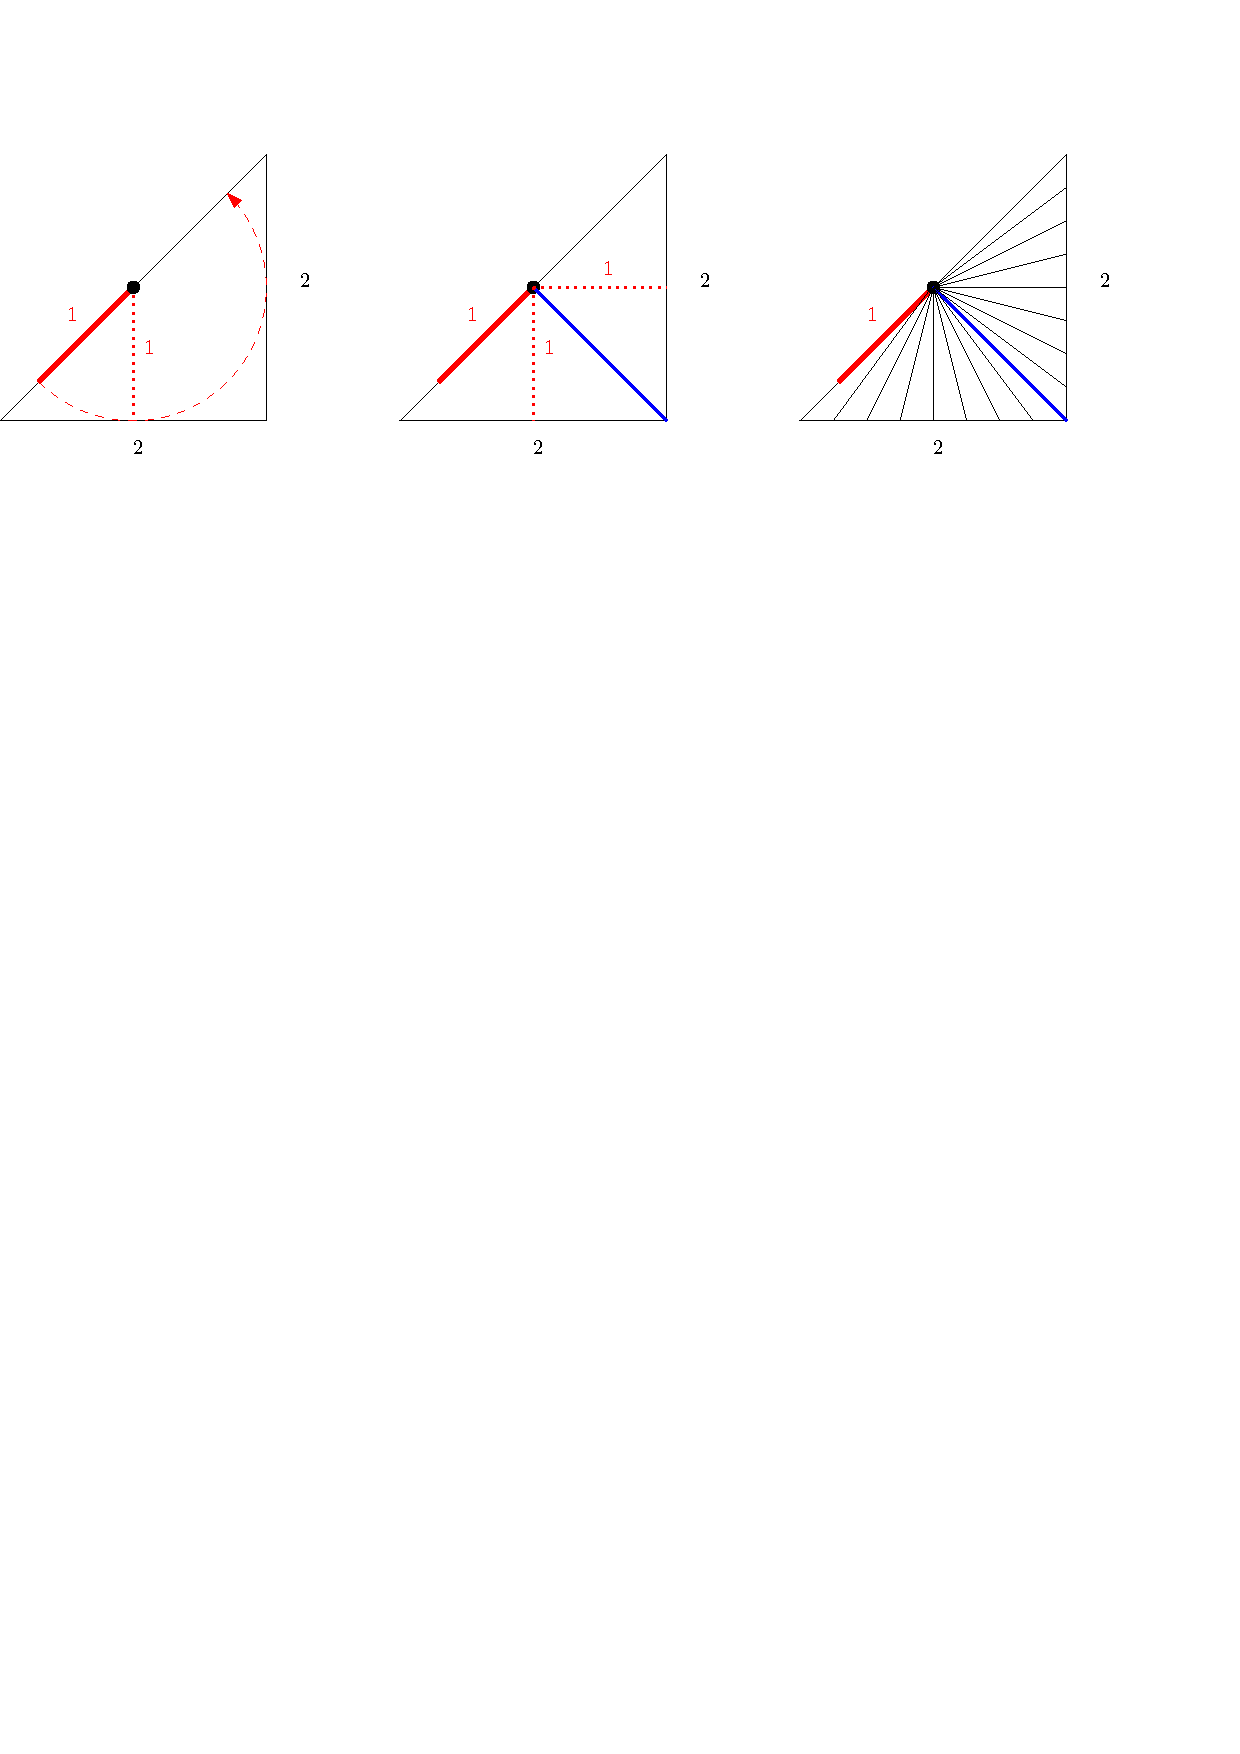
\includegraphics[width=\textwidth]{ipe_slike/trikotnik_razdelitev.pdf}
    \caption{Generiranje $ 2n $ trikotnikov z višino 1.}
    \label{trikotnik_razdelitev}
\end{figure}

\textbf{Ideja je, da se teh $ 2n $ trikotnikov tako medsebojno prekrije, da skupaj tvorijo lik z poljubno majhno ploščino, ko se $ n $ oz. število malih trikotnikov povečuje v neskončnost.}

Takoj opazimo, da se s translacijo trikotnikov ``uniči'' prehod enotske daljice iz enega trikotnika na drugega. Na sliki~\ref{preskok1} so narisane možne translacije sosednjih dveh trikotnikov. Skupne stranice so obarvane modro, enotska daljica pa z rdečo. Na levi ni spremembe in trikotnika se držita za skupno stranico, torej daljica zvezno preide iz levega trikotnika na desnega. V sredini imata trikotnika prazen presek in mora daljica na nek način iz modre stranice levega trikotnika preskočiti na modro stranico desnega ter nadaljevati svoje vrtenje. Na desni pa imamo primer prekrivanja, kjer se ravno tako pojavi vprašanje, kako daljica preskoči iz ene modre stranice na drugo.

\begin{figure}[h!]
    \centering
    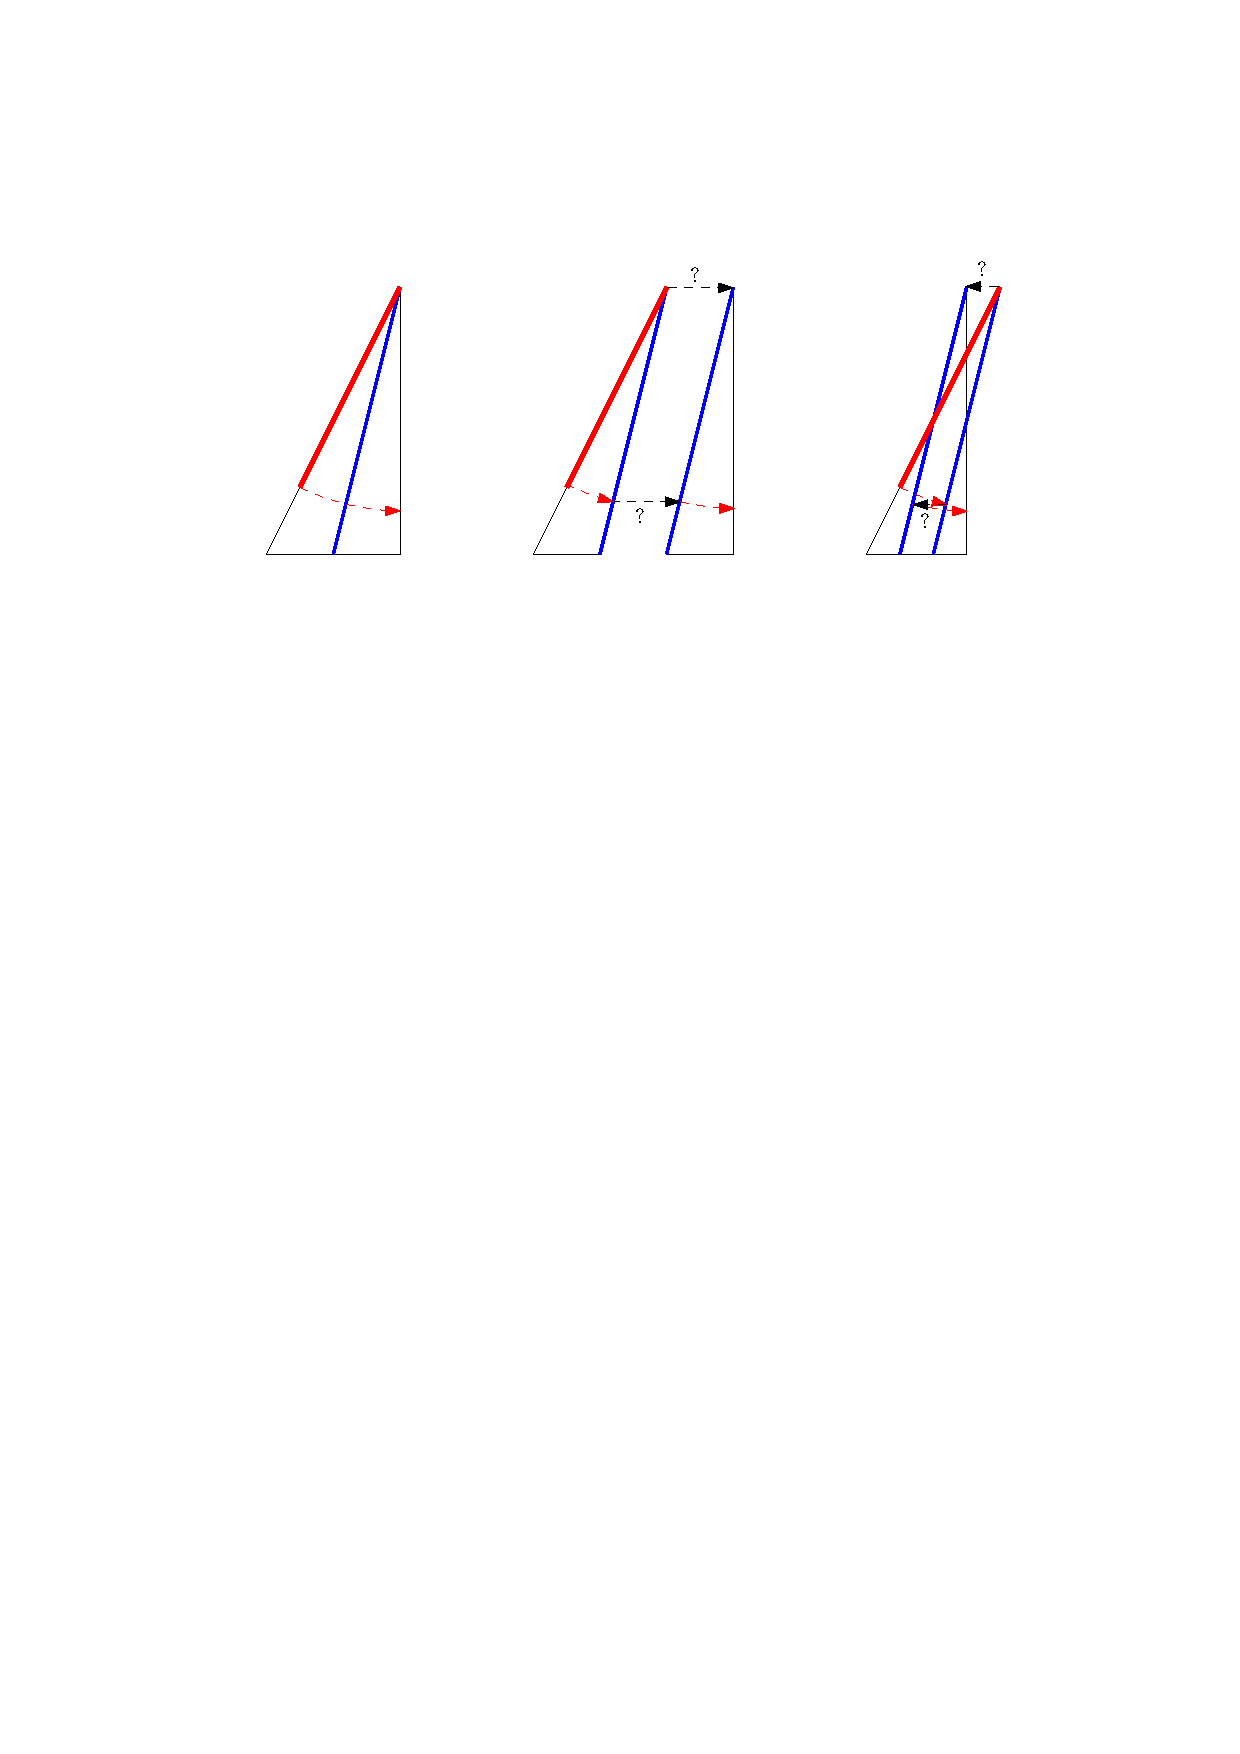
\includegraphics[width=0.7\textwidth]{ipe_slike/preskok1.pdf}
    \caption{Možne translacije sosednjih dveh trikotnikov in vrtenje daljice skozi njiju}
    \label{preskok1}
\end{figure}

%%%%%%%%%%%%%%%%%%%%%%%%%%%%%%%%%%%%%%%%%%%%%%%%%%%%%%%%%%%%%%%%%

\section*{Preskakovanje daljice med sosednjimi trikotniki}

Pál je za preskakovanje daljice med dvema sosednjima trikotnika, ki se ne stikata več na skupni stranici (sredinski in desni primer na sliki~\ref{preskok1}), podal nadvse enostavno rešitev.

Ko se enotska daljica obrne in leži na modri stranici, narišemo nosilki obeh modrih stranic. Nosilki sta seveda vzporedni. Nato zarišemo daljico, ki ju povezuje (gl. sliko~\ref{pal}). Daljico nato pošljemo po prvi nosilki do začetka povezovalne daljice, kjer jo zavrtimo okoli zgornjega krajišča, da pristane na povezovalni daljici, nato jo premaknemo po tej daljici do krajišča drugega trikotnika, jo zavrtimo v nasprotno smer in potisnemo po drugi nosilki v drugi trikotnik. Smer enotske daljice se je na ta način ohranila, daljica pa je med tem preskokom (potovanje po nosilkah ter vrtenje v krajiščih povezovalne daljice) opisala poljubno majhno ploščino, saj je kot vrtenja z daljšanjem povezovalne daljice proti neskončnosti lahko poljubno majhen ter s tem tudi orisan krožni izsek, premice pa nimajo ploščine.

\begin{figure}[h!]
    \centering
    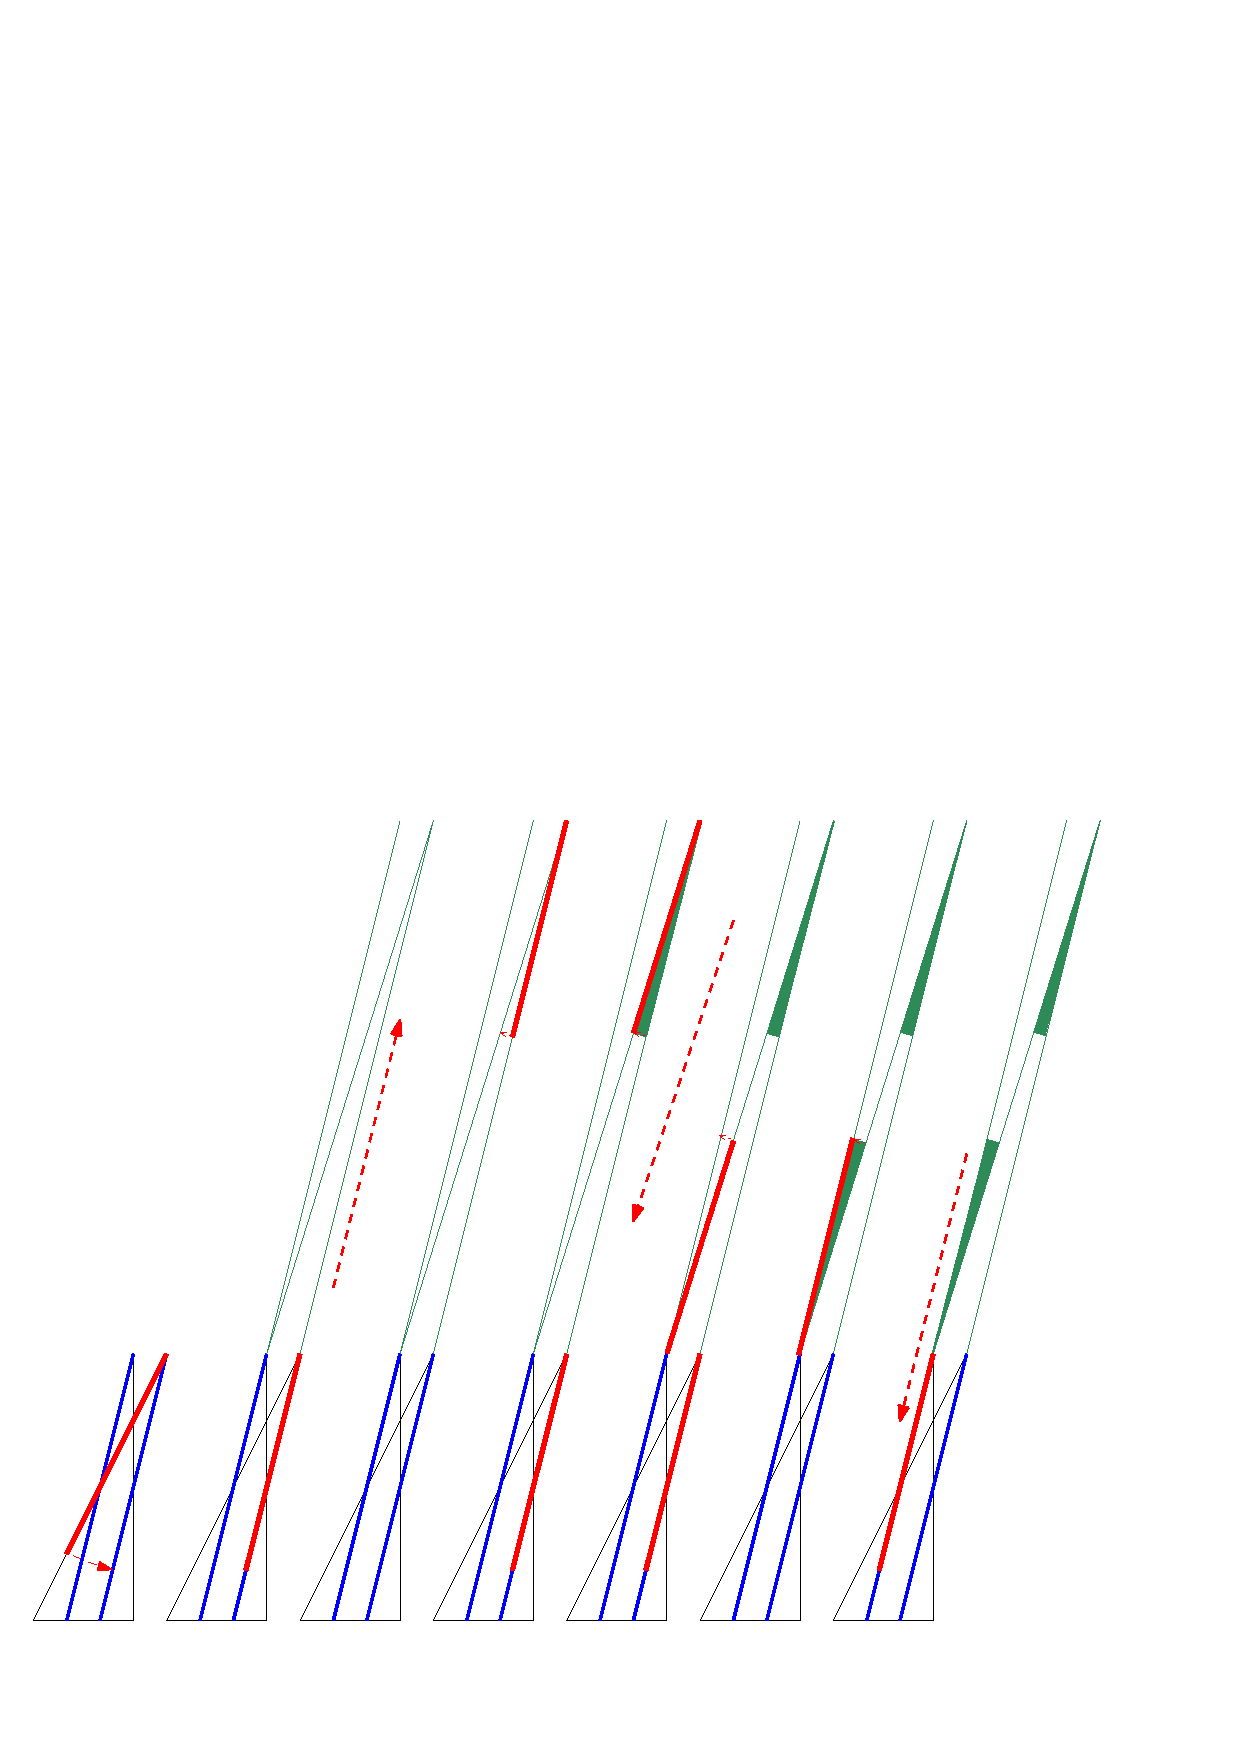
\includegraphics[width=\textwidth]{ipe_slike/pal.pdf}
    \caption{Preskok daljice med dvema prekrivajočima se sosednjima trikotnika preko lika s poljubno majhno ploščino po Pálovi zamisli}
    \label{pal}
\end{figure}

Torej za vsak preskok enotske daljice med trikotnikoma potrebujemo (in znamo konstruirati) dodatno ploščino, vendar poljubno majhno.

%%%%%%%%%%%%%%%%%%%%%%%%%%%%%%%%%%%%%%%%%%%%%%%%%%%%%%%%%%%%%%%%%


%%%%%%%%%%%%%%%%%%%%%%%%%%%%%%%%%%%%%%%%%%%%%%%%%%%%%%%%%%%%%%%%%


%%%%%%%%%%%%%%%%%%%%%%%%%%%%%%%%%%%%%%%%%%%%%%%%%%%%%%%%%%%%%%%%%

%%%%%%%%%%%%%%%%%%%%%%%%%%%%%%%%%%%%%%%%%%%%%%%%%%%%%%%%%%%%%%%%%

\section*{Zaključek}

%%%%%%%%%%%%%%%%%%%%%%%%%%%%%%%%%%%%%%%%%%%%%%%%%%%%%%%%%%%%%%%%%

% \nocite{*}      % navede tudi vire, ki jih ne citiras
\printbibliography[heading=bibintoc, title={Literatura}]

%%%%%%%%%%%%%%%%%%%%%%%%%%%%%%%%%%%%%%%%%%%%%%%%%%%%%%%%%%%%%%%%%

\end{document}